% ----------------------------------------------------------------------- %
% Arquivo: 05-API.tex
% ----------------------------------------------------------------------- %

\chapter{Interface de Aplicação} \label{cap:api}
Para demonstração dos resultados obtidos com o treinamento da rede neural, uma aplicação \textit{web} foi implementada utilizando Flask, um \textit{framework} de fácil uso que possibilita a integração com outros módulos Python.

O código desenvolvido está disponível no repositório online \url{https://github.com/anabdck/pcb-defect-detection-api} e as etapas de instalação e configuração estão no \autoref{apendice:conf-api}.

%\section{Estrutura} \label{cap:api-estrutura}
A estrutura da aplicação foi construída de acordo com o apresentado na \autoref{fig:resultados-api-estrutura}.

\begin{figure}[!h] %H
  \centering
  \caption{Estrutura da interface de aplicação proposta.}
  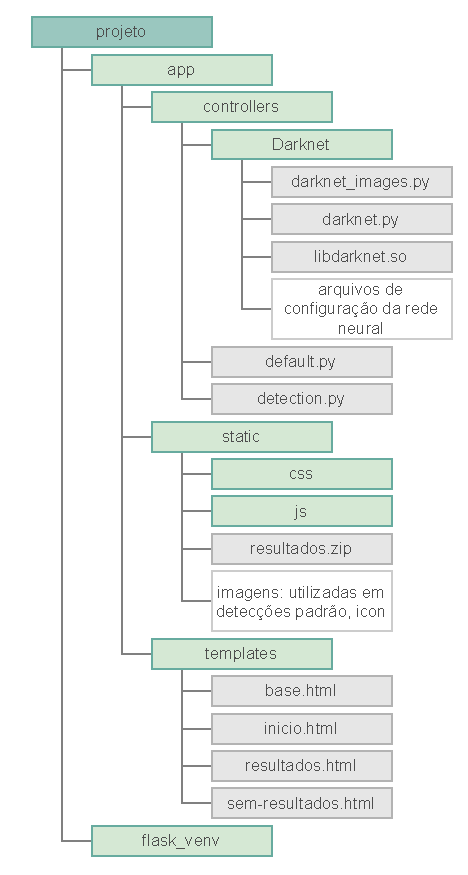
\includegraphics[scale=1.05]{img/img-resultados-api-estrutura.pdf}
  \label{fig:resultados-api-estrutura}
  \indentedfont[15.2cm]{Elaboração própria (2021)}
\end{figure}

As páginas \textit{web} apresentadas ao usuário utilizam HTML5, CSS3, Java Script e Bootstrap, organizadas dentro das pastas \textit{static} e \textit{templates} e o roteamento das páginas ocorre em \textit{default.py} dentro da pasta \textit{controllers}.


O módulo de detecção \textit{detection.py} é responsável por invocar o Darknet e processar a imagem para a detecção dos defeitos utilizando os arquivos de configuração da rede neural e os pesos treinados.
Para isso, é necessária a biblioteca \textit{libdarknet.so}, compilada para o servidor utilizado conforme o indicado nos passos do
\autoref{apendice:conf-api}.

O Fluxograma da \autoref{fig:resultados-api-etapas} apresenta de maneira abreviada as etapas de detecção dos defeitos, indicando o momento em que as diferentes páginas são renderizadas e quais são os endereços que foram roteados para a aplicação utilizados no processo.

\begin{figure}[H] %H
  \centering
  \caption{Fluxograma da detecção de defeitos de placas de circuito impresso dentro da interface de aplicação proposta.}
  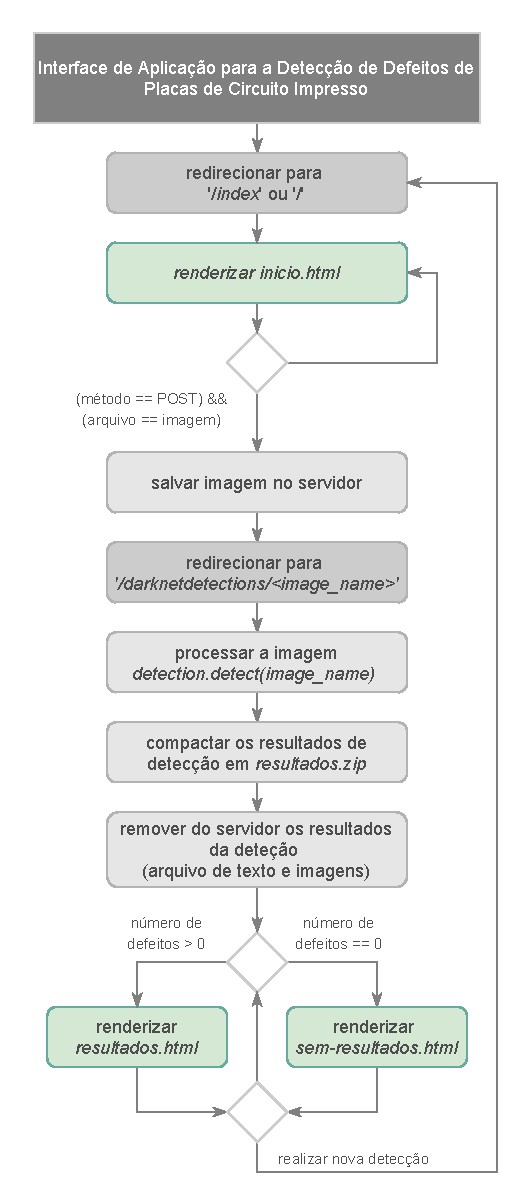
\includegraphics[scale=1.03]{img/img-resultados-api-fluxograma.pdf}
  \label{fig:resultados-api-etapas}
  \indentedfont[15.2cm]{Elaboração própria (2021)}
\end{figure}

O endereço inicial apresenta a tela da \autoref{fig:resultados-api-1}, onde o usuário pode fazer o \textit{upload} de uma imagem para a detecção ou, ao rolar a página para baixo, pode escolher uma das quatro imagens que já estão no servidor para a detecção, conforme a tela da \autoref{fig:resultados-api-2}. É possível fazer apenas o \textit{upload} de arquivos de imagens com extensões \textit{png},\textit{jpg} ou \textit{jpeg}. Caso seja feito o \textit{upload} de outros tipos de arquivos, é feito o redirecionamento para a página inicial novamente, já que as demais extensões não são aceitas pela rede neural.

Se arquivo escolhido for de uma das extensões permitidas ou o usuário escolher uma das imagens que está no servidor, a detecção dos defeitos é feita. Se a rede neural encontrar defeitos na imagem, a tela da \autoref{fig:resultados-api-3} é apresentada ao usuário, onde a indicação dos defeitos encontrados é feita por meio das caixas delimitadoras resultantes impressas na imagem processada. Uma mensagem indicando o tempo de processamento e a quantidade de defeitos encontrados é exibido ao usuário. O botão de ``\textit{Download} dos Resultados'' salva no computador do usuário um arquivo compactado contendo a imagem com as caixas delimitadoras e um arquivo de texto de anotação no padrão YOLO. Caso nenhum defeito é encontrado, a imagem original é mostrada ao usuário, além do aviso indicando o tempo de processamento, conforme a \autoref{fig:resultados-api-5}. O botão de ``\textit{Download} dos Resultados'' fica travado nesse caso.

A aplicação construída não considerou o uso de GPUs, mas caso esteja disponível no servidor utilizado, o Darknet pode ser compilado para isso, melhorando o tempo de processamento da detecção que para o servidor testado varia em torno de vinte segundos.

\begin{landscape}
  \begin{figure}[H] %H
    \centering
    \caption{Tela Inicial 1 da Interface de Aplicação.}
    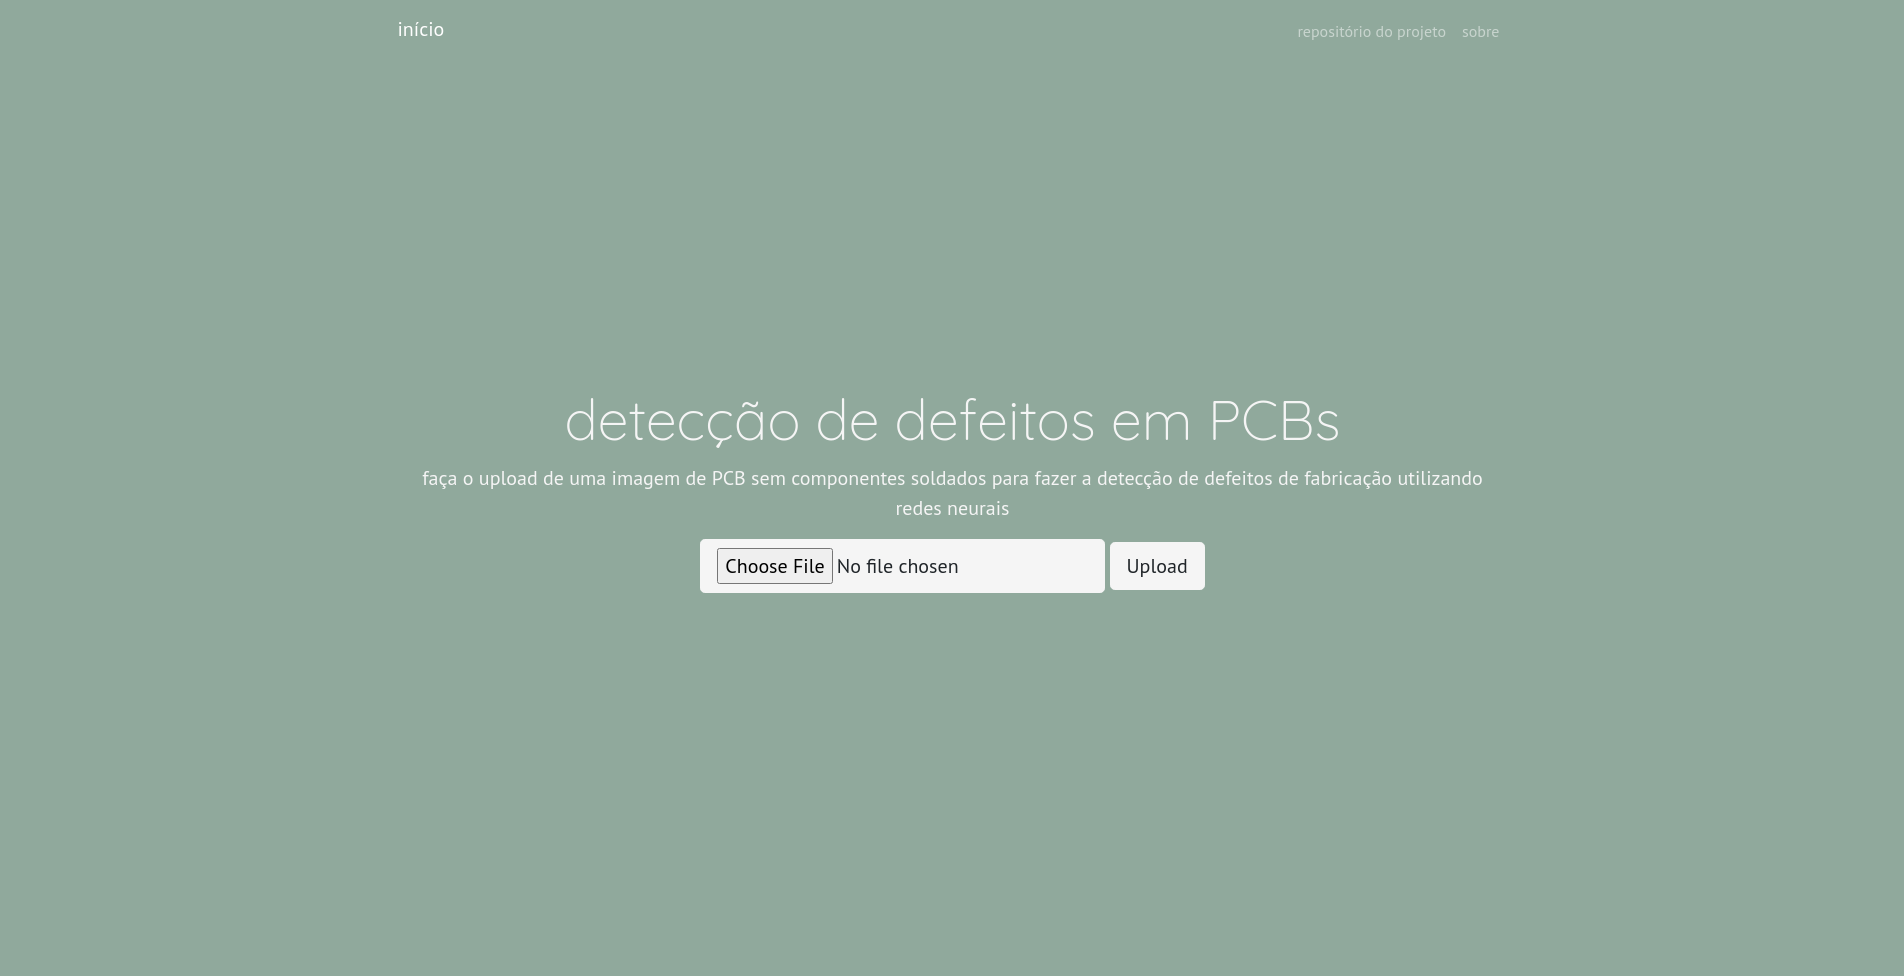
\includegraphics[scale=0.36]{img/api/1.png}
    \label{fig:resultados-api-1}
    \indentedfont[15.2cm]{Elaboração própria (2021)}
  \end{figure}
\end{landscape}

\begin{landscape}
  \begin{figure}[H] %H
    \centering
    \caption{Tela Inicial 2 da Interface de Aplicação.}
    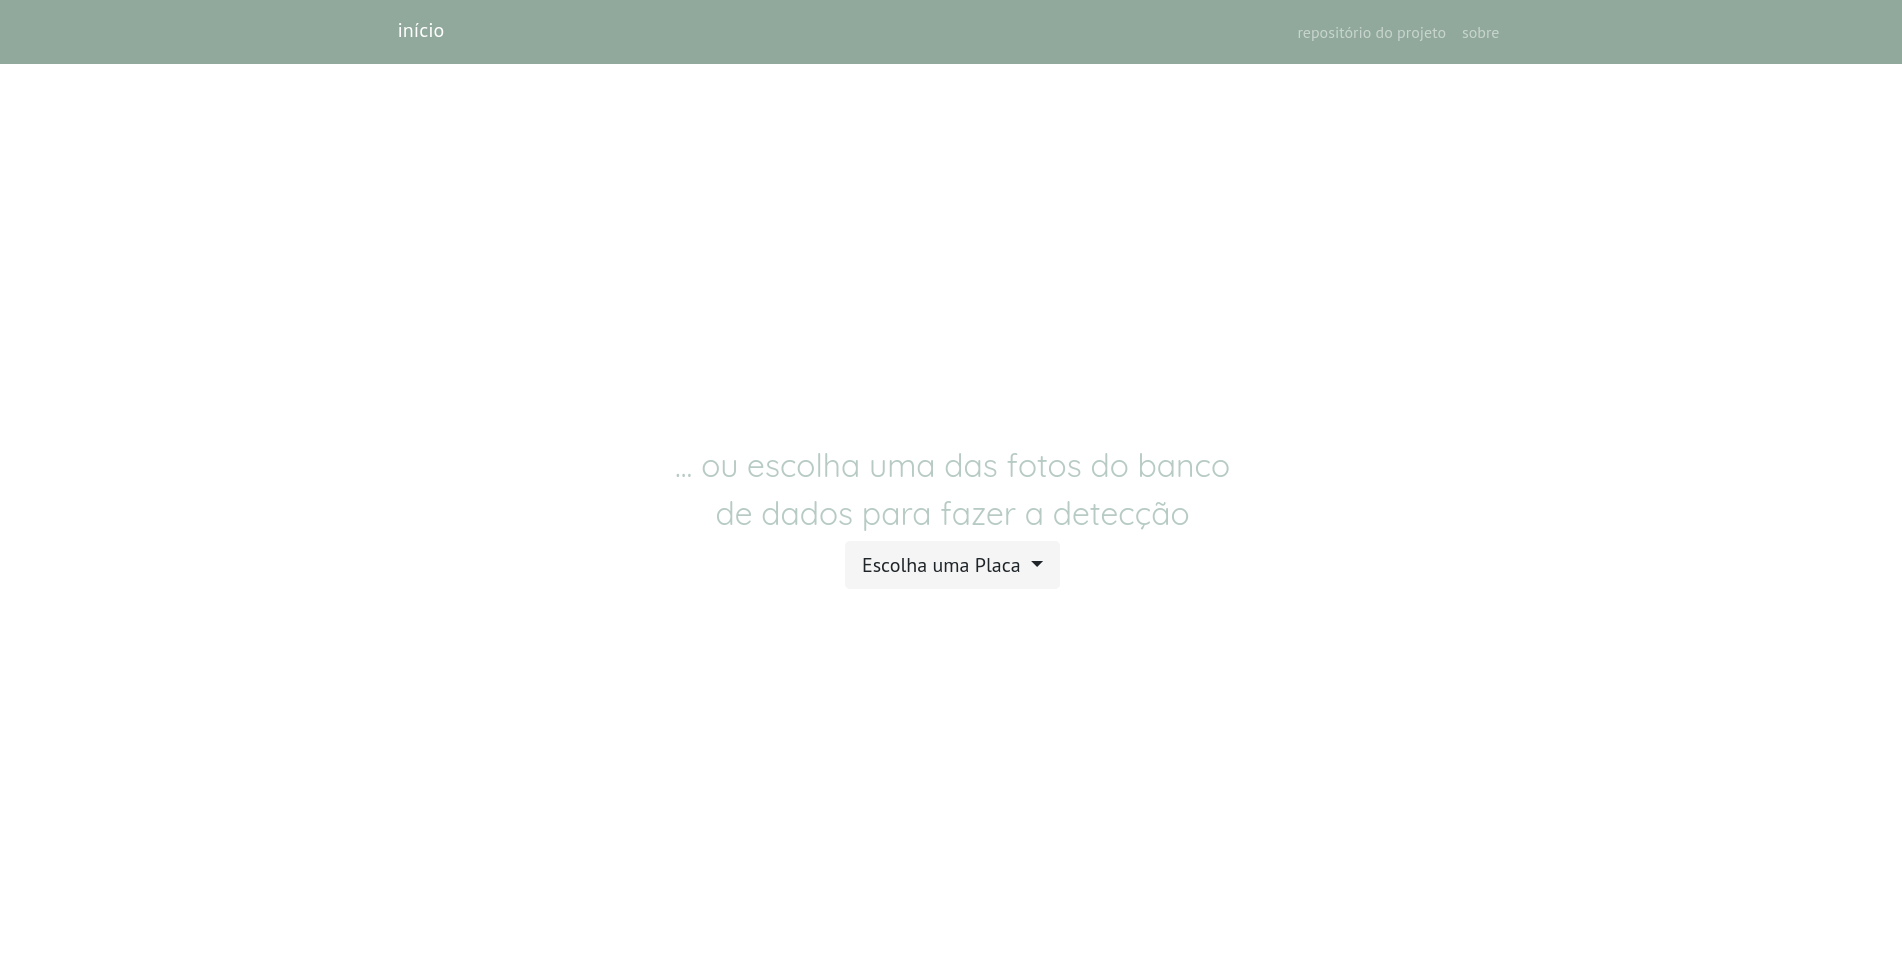
\includegraphics[scale=0.36]{img/api/2.png}
    \label{fig:resultados-api-2}
    \indentedfont[15.2cm]{Elaboração própria (2021)}
  \end{figure}
\end{landscape}

\begin{landscape}
  \begin{figure}[H] %H
    \centering
    \caption{Tela da Interface de Aplicação para imagem com detecções.}
    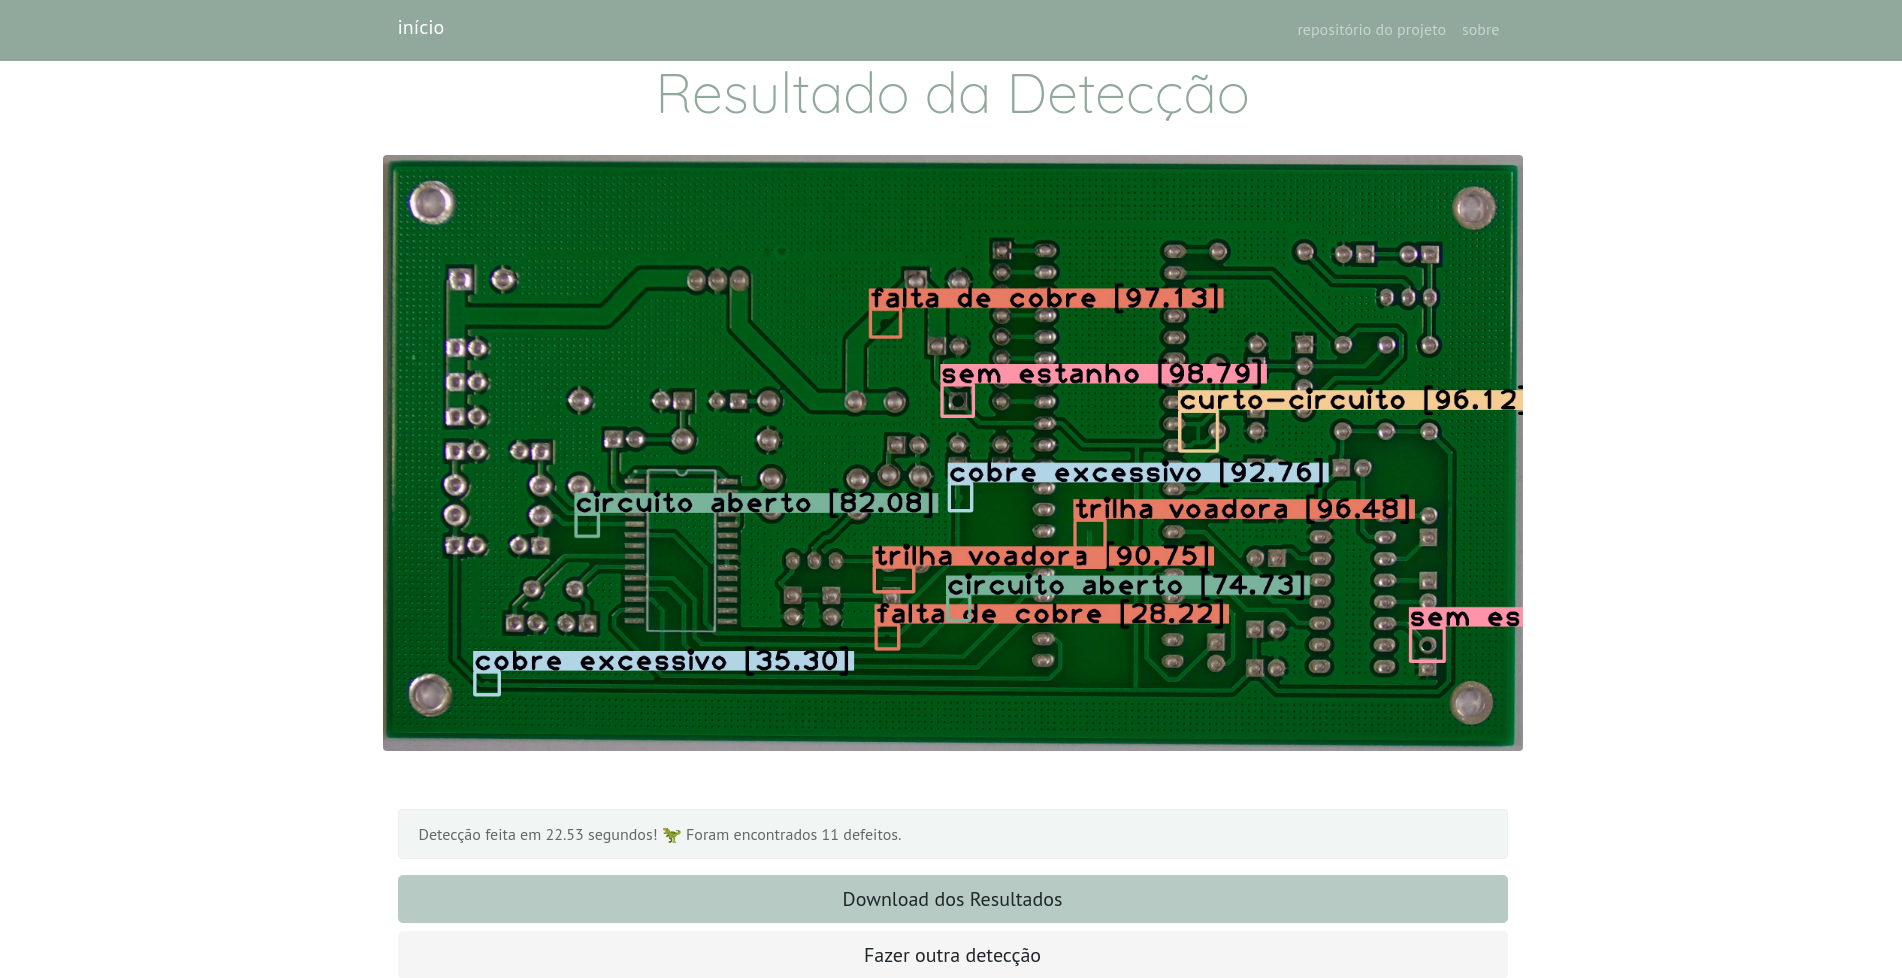
\includegraphics[scale=0.36]{img/api/3.png}
    \label{fig:resultados-api-3}
    \indentedfont[15.2cm]{Elaboração própria (2021)}
  \end{figure}
\end{landscape}

\begin{landscape}
  \begin{figure}[H] %H
    \centering
    \caption{Tela da Interface de Aplicação para imagem sem detecções.}
    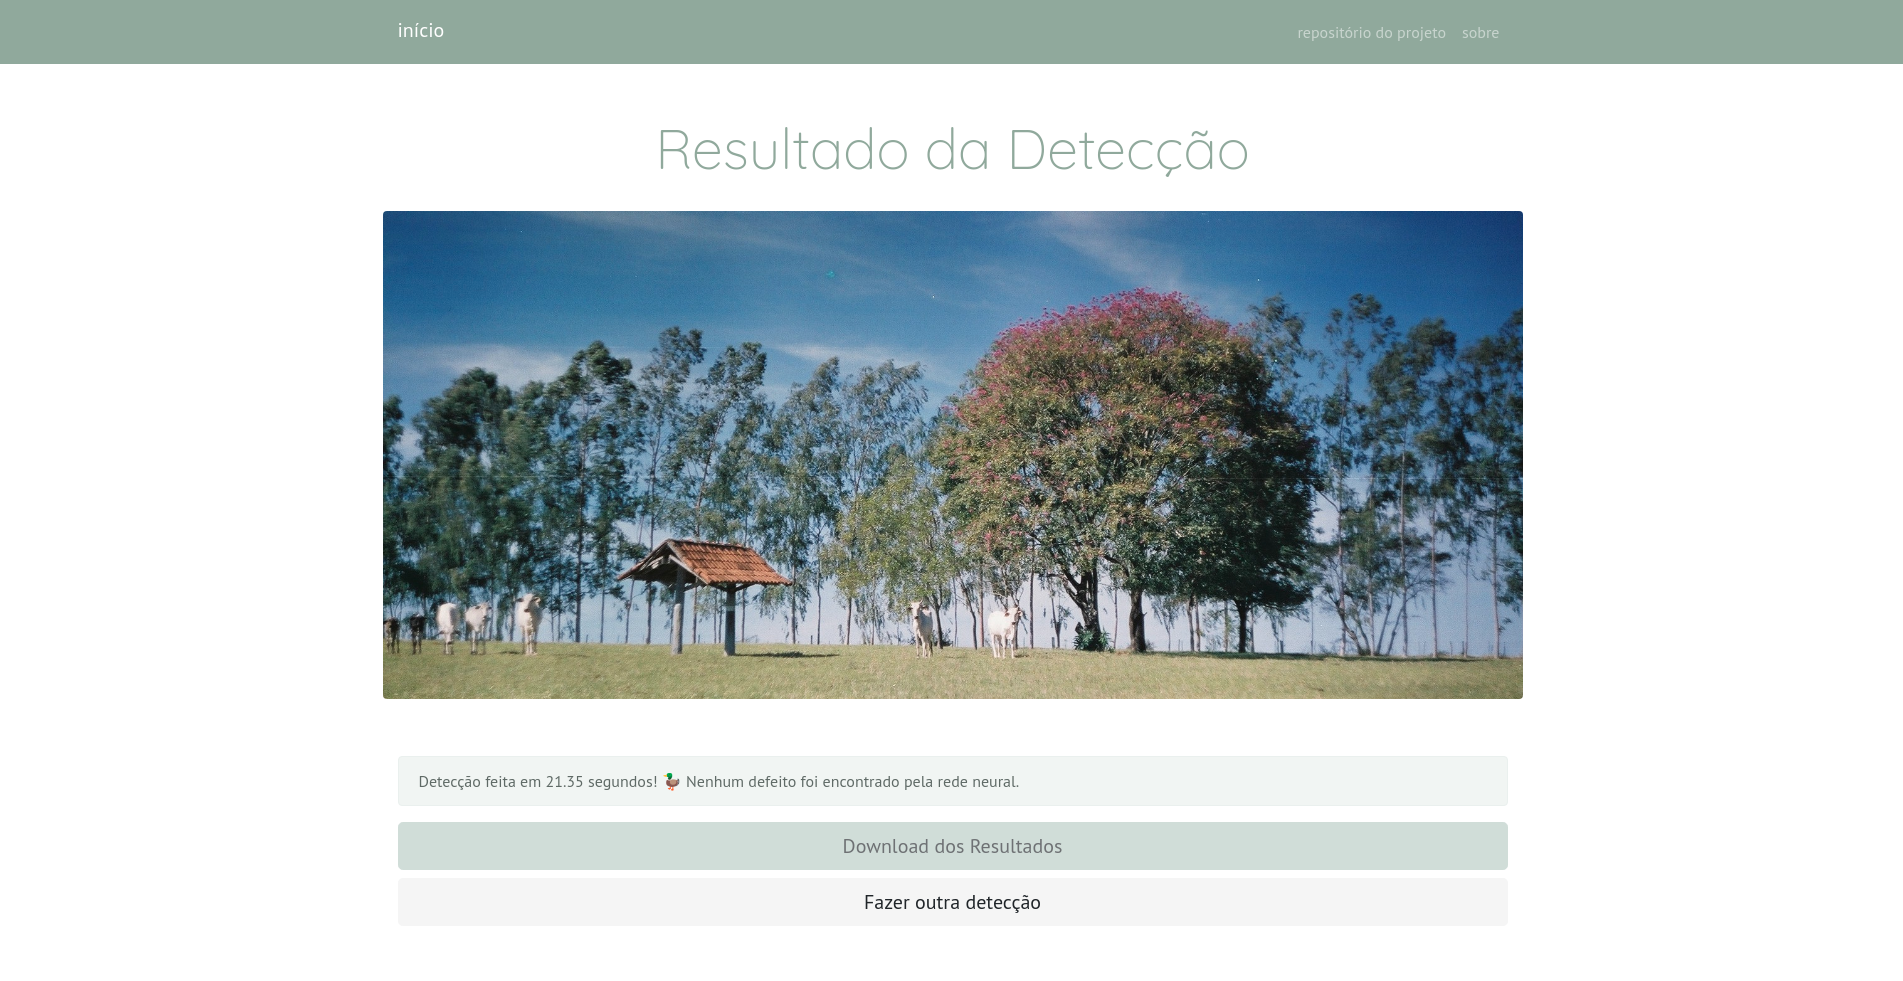
\includegraphics[scale=0.36]{img/api/5.png}
    \label{fig:resultados-api-5}
    \indentedfont[15.2cm]{Elaboração própria (2021)}
  \end{figure}
\end{landscape}
